\documentclass[conference]{IEEEtran}
\IEEEoverridecommandlockouts
% The preceding line is only needed to identify funding in the first footnote. If that is unneeded, please comment it out.
\usepackage{cite}
\usepackage{amsmath,amssymb,amsfonts}
\usepackage{algorithmic}
\usepackage{graphicx}
\usepackage{textcomp}
\usepackage{xcolor}
\usepackage{float}
\usepackage{placeins}
% \def\BibTeX{{\rm B\kern-.05em{\sc i\kern-.025em b}\kern-.08em
%     T\kern-.1667em\lower.7ex\hbox{E}\kern-.125emX}}
\begin{document}

\title{Git Operations: Argo CD vs Flux\\}

\author{\IEEEauthorblockN{Author: Qadeer Hussain}
\and
\IEEEauthorblockN{Course: Software Development Yr 4}
\texttt{18/05/2025}
\and
\IEEEauthorblockN{Module: Cloud Data Centres Report}
}
\maketitle

\begin{abstract}
This report covers Git Operations, a modern approach to continuous deployment using Git as the source of truth. It compares two popular Git Ops tools Argo CD and Flux and demonstrates their use in Kubernetes environments. A hands on example with Argo CD is included to illustrate practical implementation.
\end{abstract}

\begin{IEEEkeywords}
Git Ops, Argo CD, Flux, Continuous Deployment (CD), Kubernetes, Git Repositories 
\end{IEEEkeywords}

\section{Introduction}
This report focuses on Git Operations, explaining its definition and relevance to cloud native computing. It also examines two widely used Git operation tools: Argo CD and Flux.

\section{What is Git Operations}
Git Operations is a way of implementing Continuous Deployment for Cloud Applications. The main idea of Git Ops is to have a Git repository that has declarative descriptions of the infrastructure currently in the production environment and an automated process to make the production environment match the described state in the repository. [1][2][3]

Git Ops has many benefits, such as efficiency, security, reduced costs, and faster deployments. Git Ops helps organisations manage containers and micro services more effectively by using Kubernetes, while maintaining consistency across all their infrastructure. [2][8]

\section{Git Ops Workflow}
The Git Ops workflow is built around four components each playing vital role in deployment and management of applications.

\begin{itemize}
    \item \textbf{Git Repository:} Acts as the central source of truth for both applications code and configuration. Stores all critical information in the repository. [2]
    
    \item \textbf{Continuous Delivery (CD) Pipeline:} CD pipeline automates process of building, testing and deploying. Facilitating a smooth transition from development to production environments. [2]
    
    \item \textbf{Application Deployment Tool:} In charge of deploying the application to the desired environment. Orchestrates and manages the applications resources, making sure the application is deployed correctly and efficiently according to the configuration of the git repository. [2]

    \item \textbf{Monitoring System:} This is needed for maintaining the applications health, the system, keeps an eye on the applications performance. Gathers data and provides the development team with insight and feedback allowing them to make decisions based on any issues that arise. [2]
\end{itemize}

\begin{figure}[htbp]
    \centering
    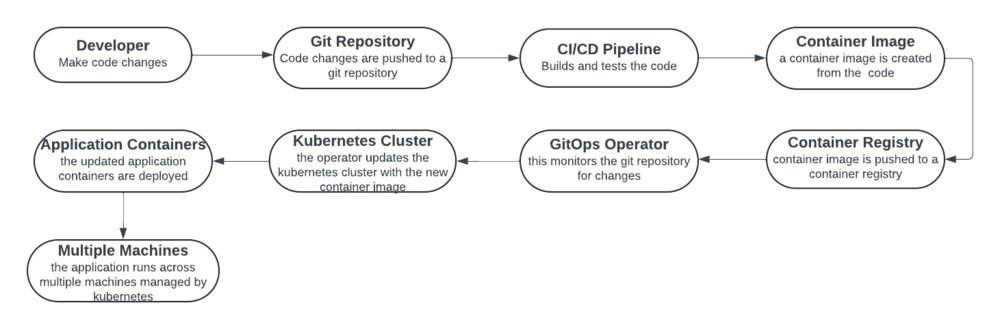
\includegraphics[width=1\linewidth]{Git Ops WorkFlow.png}
    \caption{Git Ops Workflow}
    \label{fig:gitops-workflow}
\end{figure}

\section{Overview of Git Ops Tools}
There are several tools used to support Git Ops workflows by automating deployment and synchronisation between Git repositories and Kubernetes clusters. Among them most widely adopted are Argo CD and Flux, both which allow for continuous Deployment using Git as the source truth. [2]

\section{Argo CD}

\begin{figure}[htbp]
    \centering
    
\includegraphics[width=0.35\linewidth]{ArgoCDImage.png}
    \caption{Argo CD}
    \label{fig:argo-cd}
\end{figure}

\subsection{Overview}
Argo CD is a declarative open source, Git Ops continuous delivery tool for Kubernetes. It is a part of the Cloud Native Computing Foundation (CNCF). The aim of Argo CD is to automate deployment of applications into specific target environments inside of Kubernetes, using Git Repository as the source of truth for the desired state of applications. [6][7][8]

Continuously monitors Git repositories and compares the states of the application defined in the repository with the actual state in Kubernetes environment. Any differences noted trigger an automatic sync to ensure the actual state matches the desired state. By doing this, Argo CD provides a level of automation and control that dramatically simplifies management of deployments in Kubernetes. [6][7][8] 

Argo CD has a comprehensive dashboard which provides visual representation of the applications status allowing for easy management. Also provides access control, audit logs and supports a range of configurations tools such as Kustomize, Helm. [6][7][8] 

\subsection{Argo Architecture}
The core components of Argo CD include the API Server, Repository Server, and Application Controller:
\begin{itemize}
    \item \textbf{API Server:} Is a gRPC/REST server which exposes API consumed by Web UI, CLI and CI/CD systems. It handles application management, status reporting, invoking of application operations, repository and cluster credential management, authentication and auth delegation, RBAC enforcement and listener/forwarder for Git web hook events. [4]
    
    \item \textbf{Repository Server:} Maintains a local cache of Git repositories and is responsible for generating Kubernetes manifests from the application's source, using inputs such as the repository URL, revision, application path and template specific settings. [4]
    
    \item \textbf{Application Controller:} Continuously monitors the state of deployed applications and compares it with the desired state from the repository. It detects OutOfSync application state and takes action. Responsible for invoking user-defined hooks for lifecycle events such as Pre Sync, Sync and Post Sync. [4]
\end{itemize}

\begin{figure}[htbp]
    \centering
    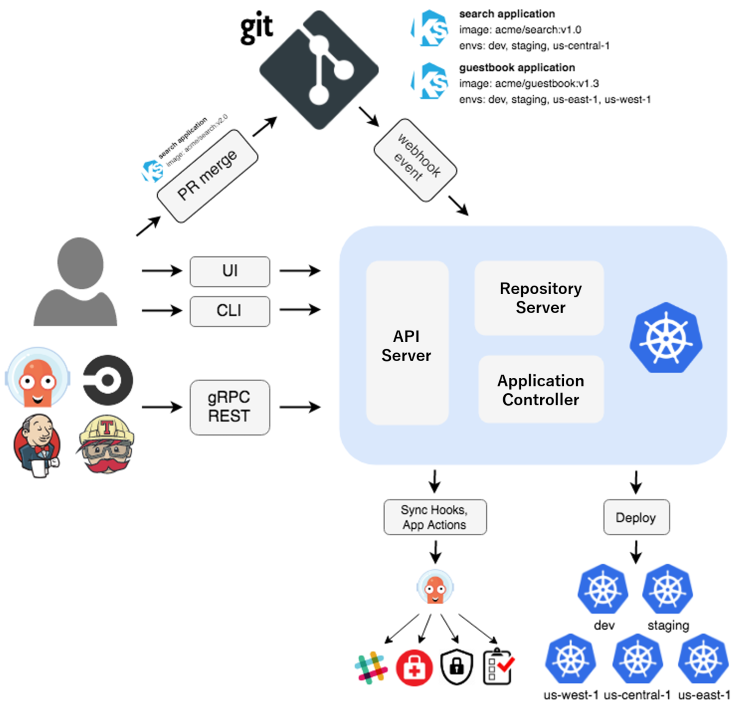
\includegraphics[width=0.7\linewidth]{Argo_CD_Architecture.png}
    \caption{Argo CD Architecture}
    \label{fig:argo-cd-arch}
\end{figure}

\section{Flux}

\begin{figure}[htbp]
    \centering
    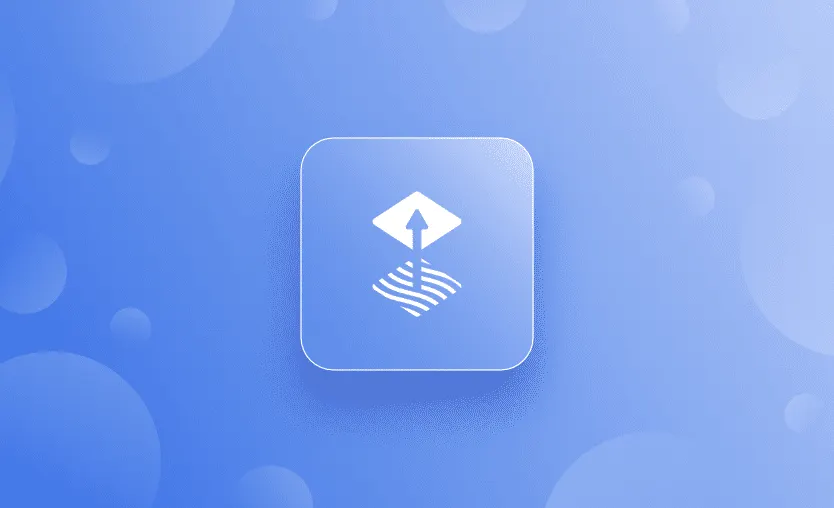
\includegraphics[width=0.5\linewidth]{FluxImage.png}
    \caption{Flux}
    \label{fig:flux}
\end{figure}

\subsection{Overview}
Flux is another open source tool for Git Ops which is also designed to implement Git Ops workflows in Kubernetes. Just like Argo CD Flux is also apart of the Cloud Native Computing Foundation (CNCF). [6][7][8]

Flux operates in a very similar manner to Argo CD it also continuously monitors Git repositories and compares the states of the application defined in the repository with the actual state in Kubernetes environment. Any differences noted trigger an automatic sync to ensure the actual state matches the desired state. Flux also has image updates, automatically tracking and deploying containers images, this makes it useful for continuous delivery. [6][7][8] 

Flux like Argo also supports similar configuration tools such as Kustomize, Helm. Key features include automated roll outs, rollbacks, and multi-environment support. [6][7][8]

\subsection{Flux Architecture}
Flux is designed to run within Kubernetes. It relies heavily on native resources and API's. This approach allows for more granular control and flexibility. However, this requires additional setup for a complete overview. This external tools like Weave Git Ops for visualisation. [7][8]

\begin{figure}[htbp]
    \centering
    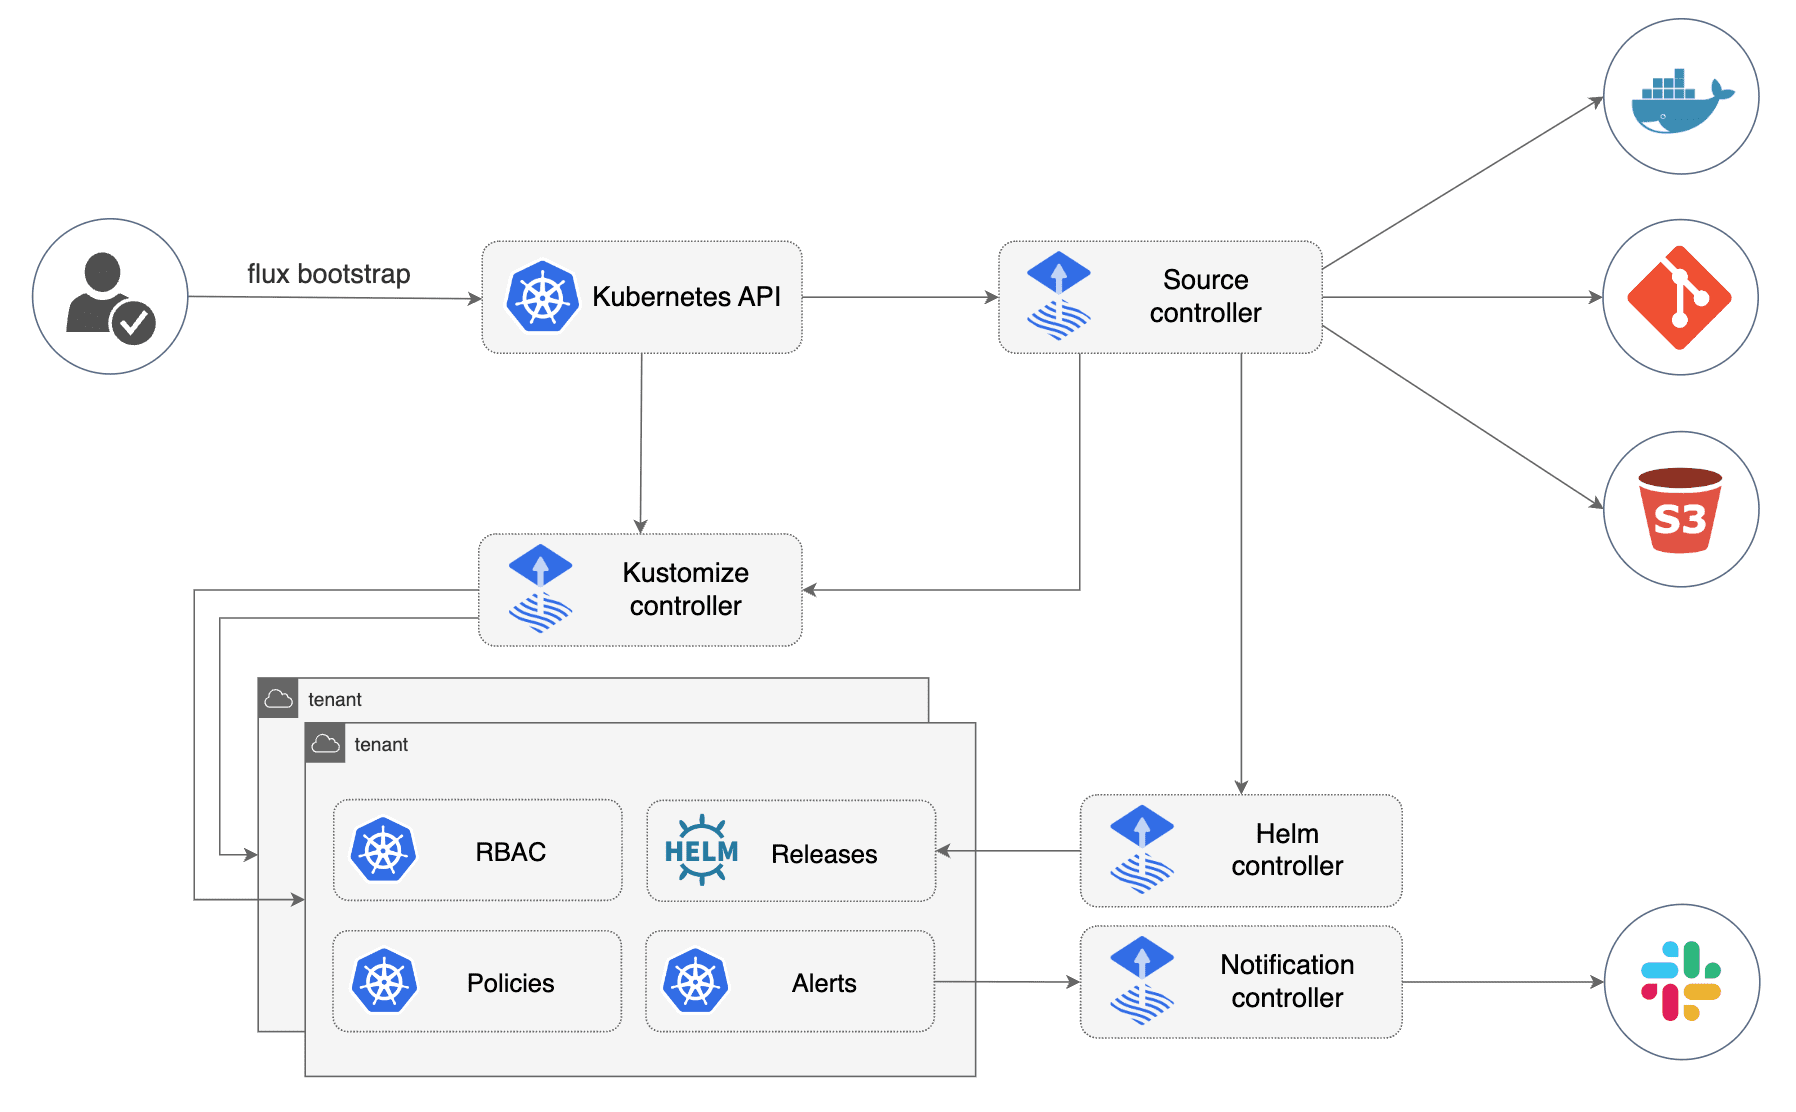
\includegraphics[width=0.7\linewidth]{Flux Architecture.png}
    \caption{Flux Architecture}
    \label{fig:flux-arch}
\end{figure}

\section{Comparison}

\subsection{Architecture}
Both Argo CD and Flux are similar in there uses and function. However, Flux, is heavily dependent on Kubernetes resources and API's. This allows for more control and flexibility but requires additional setup for complete overview. Flux is an expandable toolkit, whereas, Argo CD is a complete application. Therefore, Argo is more opinionated then Flux. [7][8]  

\subsection{Development Process}
Flux and Argo CD offer same deployment processes. Register the application using CLI or Kubernetes CRD's, stating the source to connect to such as the git repository. The tools get the state from the repository and position the application in the cluster. When an update is ready to be applied, push it to the repository. The tool will sync changes into the cluster, manually or automatically. Flux and Argo CD support Kustomize templates Helm charts. However, Argo does not use Helm internally, as Helm has some difficulties such as its awkwardness with CRD management. [8]

\subsection{Declarative Configuration}
Flux and Argo CD both support declarative configuration. Flux favours Git Repository and Kustomisation. While Argo favours high abstraction with applications and applications sets. Declarative Configuration is used by flux to manage installation in the cluster. When Flux is installed it must specify or create  a git repository that will store config manifests used by Flux. One can reproduce the same environment with this process. [8]

\subsection{Ease of use}
Flux and Argo CD are easy to implement use as they are supported by robust CLI and clear documentation. However, Flux has lower-level config mechanism and a steeper learning curve then Argo CD. Argo is more accessible with in built web interface. [8]

\subsection{Access Management}
Flux does not have its own access management system. Kubernetes identify, and RBAC controls must be used to configure who can interact with Flux resources. This standardises all controls in Kubernetes RBAC mechanism, however it makes it difficult to enforce granular policies. Argo allows the user to decouple access control from cluster level Kubernetes users. Argo users can be created by adding 'local' users to config map. Once the user is added, actions can be performed with Argo's RBAC layer. [8]

\section{Implementation: Argo CD Hands-On Deployment}
\subsection{Install Argo CD}
\begin{figure}[htbp]
    \centering
    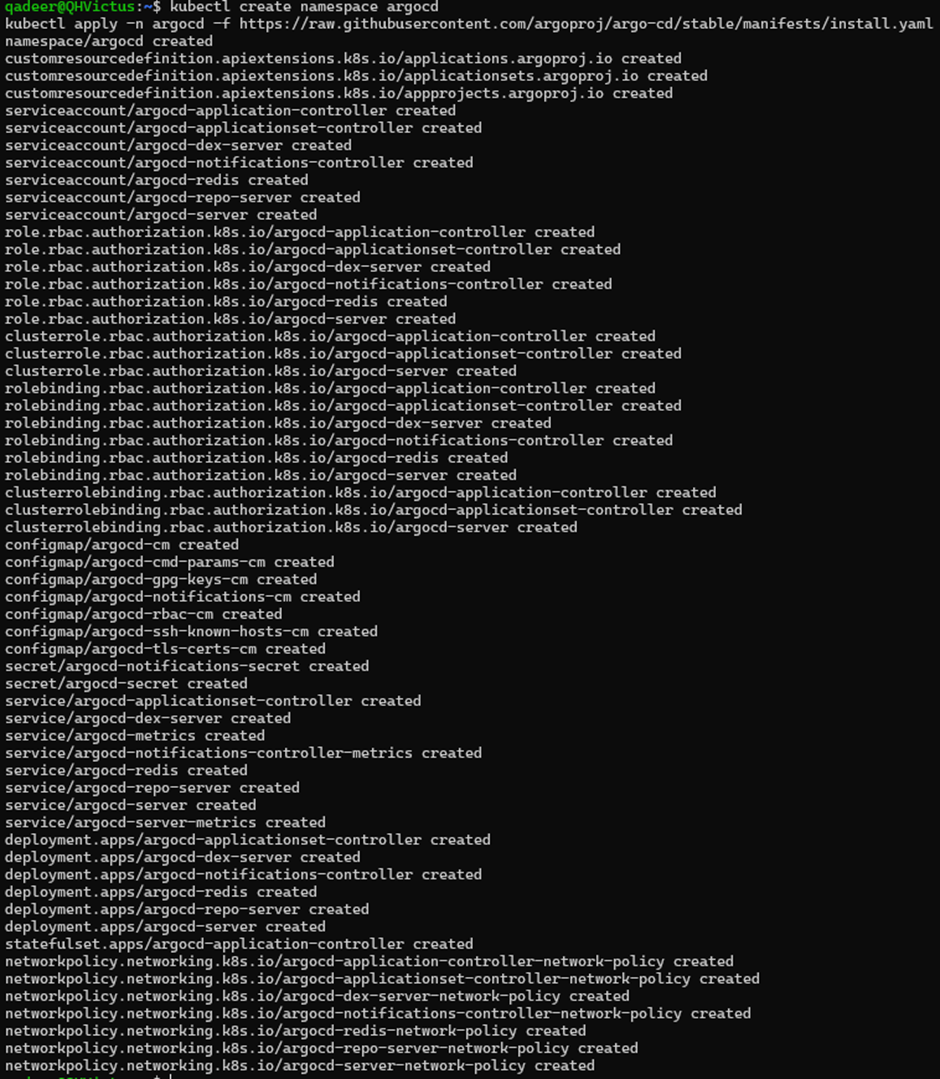
\includegraphics[width=0.8\linewidth]{Install Argo CD.png}
    \caption{Install Argo}
    \label{fig:install-argo-cd}
\end{figure}

\subsection{Service Type Load Balancer}
\begin{figure}[htbp]
    \centering
    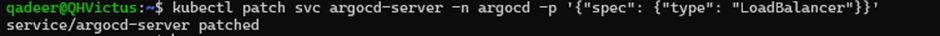
\includegraphics[width=1\linewidth]{Service Type Load Balancer.png}
    \caption{Service Type Load Balancer}
    \label{fig:service-type-load-balancer}
\end{figure}

\subsection{Port Forwarding}
\begin{figure}[htbp]
    \centering
    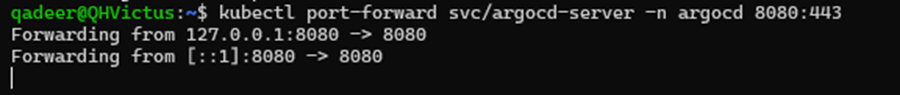
\includegraphics[width=1\linewidth]{Port Forwarding.png}
    \caption{Port Forwarding}
    \label{fig:port-forwarding}
\end{figure}

\subsection{Login Using The CLI}
\begin{figure}[htbp]
    \centering
    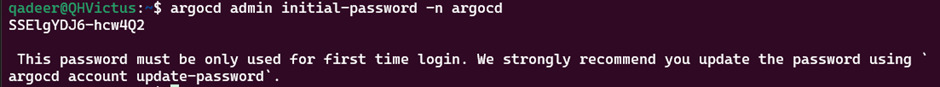
\includegraphics[width=1\linewidth]{Get Password.png}
    \caption{Get Password}
    \label{fig:get-password}
\end{figure}

\begin{figure}[htbp]
    \centering
    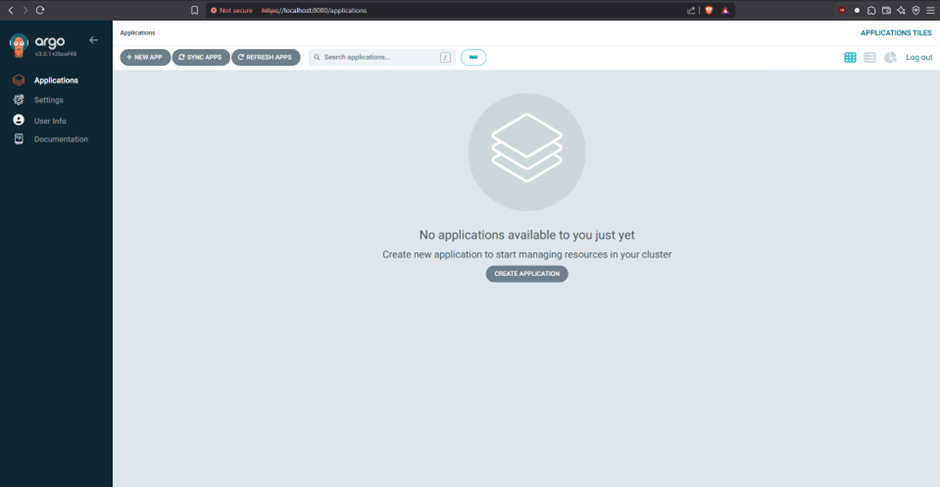
\includegraphics[width=1\linewidth]{Logged into Argo.png}
    \caption{Logged into Argo}
    \label{fig:logged-in}
\end{figure}

\subsection{Creating Apps via CLI}
\begin{figure}[H]
    \centering
    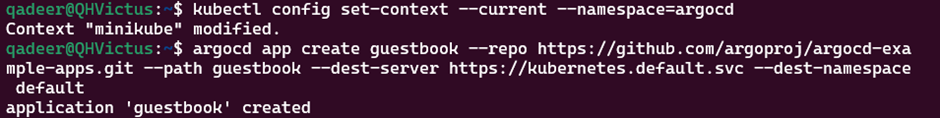
\includegraphics[width=1\linewidth]{Creating Apps via CLI 1.png}
    \caption{Creating Apps via CLI 1}
    \label{fig:creating-apps-via-cli-1}
\end{figure}

\begin{figure}[H]
    \centering
    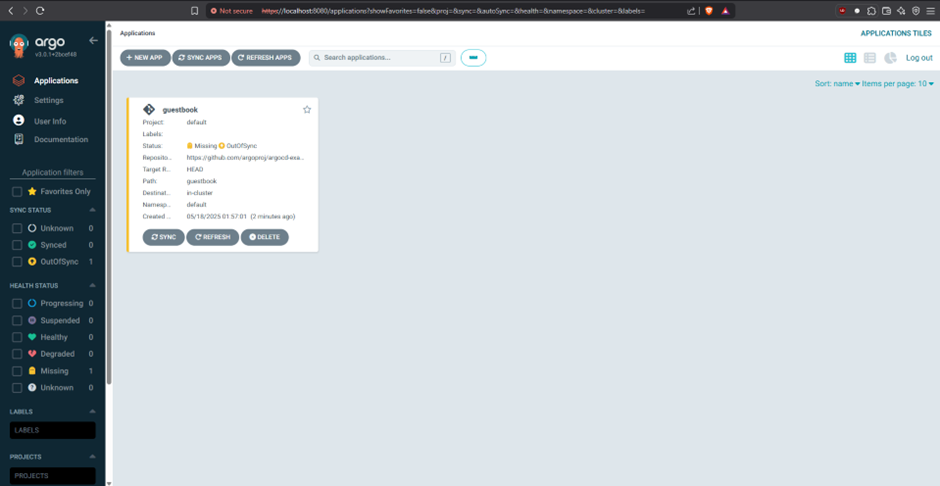
\includegraphics[width=1\linewidth]{Creating Apps via CLI 2.png}
    \caption{Creating Apps via CLI 2}
    \label{fig:creating-apps-via-cli-2}
\end{figure}

\subsection{Creating Apps via UI}
\begin{figure}[htbp]
    \centering
    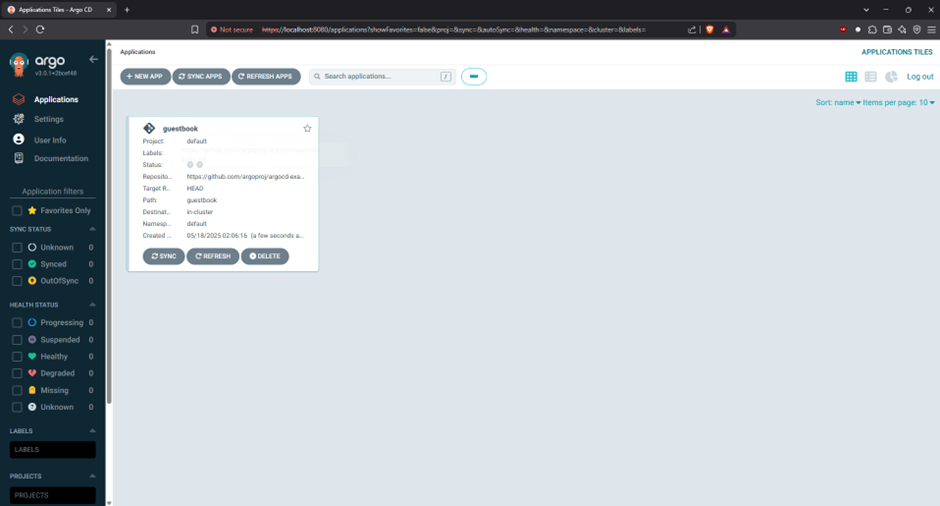
\includegraphics[width=1\linewidth]{Creating Apps Via UI.png}
    \caption{Creating Apps Via UI}
    \label{fig:creating-apps-via-UI}
\end{figure}

\subsection{Sync (Deploy) The Application}
\begin{figure}[htbp]
    \centering
    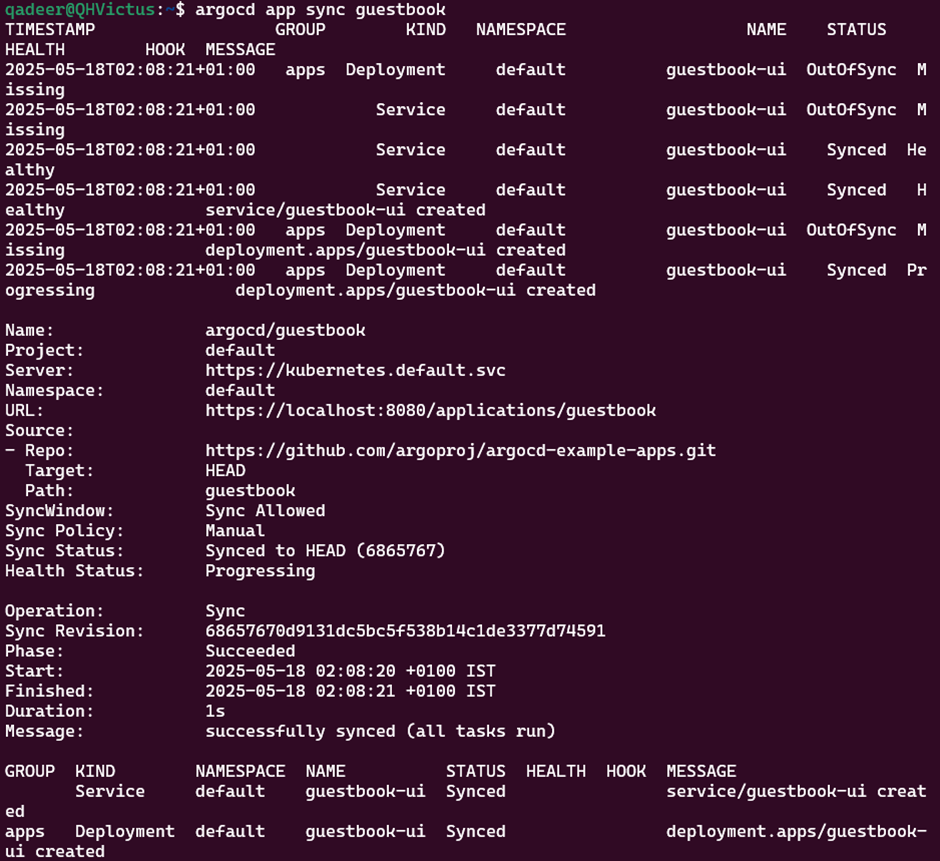
\includegraphics[width=1\linewidth]{Syncing via CLI.png}
    \caption{Syncing via CLI}
    \label{fig:sync-via-cli}
\end{figure}

\subsection{Syncing via UI}
\begin{figure}[H]
    \centering
    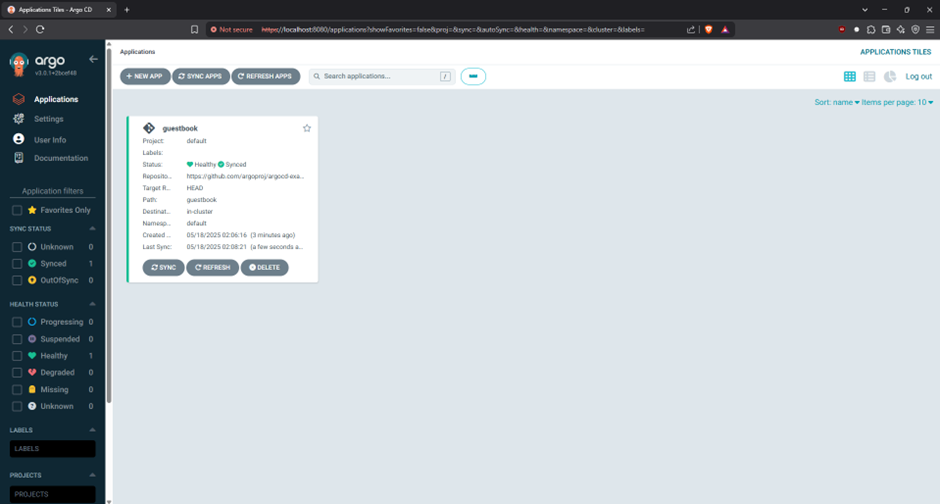
\includegraphics[width=1\linewidth]{Syncing via UI 1.png}
    \caption{Syncing via UI 1}
    \label{fig:sync-via-ui-1}
\end{figure}

\begin{figure}[htbp]
    \centering
    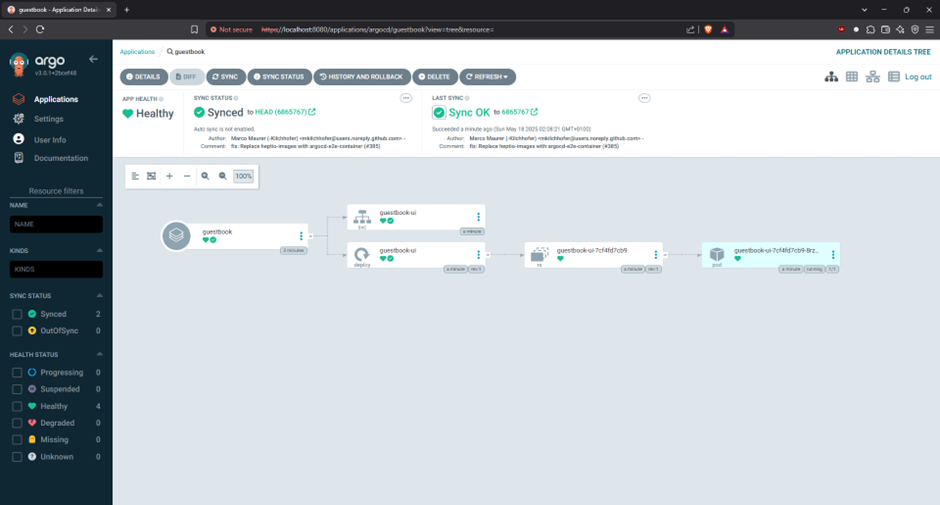
\includegraphics[width=1\linewidth]{Syncing via UI 2.png}
    \caption{Syncing via UI 2}
    \label{fig:sync-via-ui-2}
\end{figure}

\section{Challenges}
The following challenges were encountered during the research and practical implementation: 

\begin{itemize}
    \item {One of the main challenges was researching recent comparisons between Argo CD and Flux. Many online resources vary in depth and focus. Filtering through the documents and cross referencing sources.}

    \item{During the Argo CD setup, a few issues were encountered due to outdated commands found in third-party sources. To resolve this, the official Argo CD documentation was used to ensure command accuracy and version compatibility. The setup process was further streamlined by experience with Kubernetes through earlier labs.}
    
\end{itemize}

\section{Conclusion}
In conclusion this report examined the basis of what Git Operations is and covered two popular Git Ops tools Argo CD and Flux. While both tools offer similar core functionality, they differ in architecture, ease of use, and flexibility. Argo CD provides a more user-friendly experience with a built-in UI. Flux, on the other hand, offers greater flexibility appealing to users who prefer a more Kubernetes-native and extensible setup.

Through a hands on use of Argo CD, this report illustrated how Git Ops can be effectively implemented in practice. As organisations continue to scale their cloud infrastructure, adopting Git Ops practices with the right tool can significantly improve deployment and management.

\begin{thebibliography}{00}
\bibitem{b1}A. K. S. H. Florian Beetz, “GitOps,” [Online]. Available: https://www.gitops.tech/. [Accessed May 2025].
\bibitem{b2}GitLab, "What is GitOps?," 2025. [Online]. Available: https://about.gitlab.com/topics/gitops/. [Accessed May 2025].
\bibitem{b3}Geekas For Geeks, "Continuous Deployment to Kubernetes with GitOps," July 2024. [Online]. Available: https://www.geeksforgeeks.org/continuous-deployment-to-kubernetes-with-gitops/. [Accessed May 2025]
\bibitem{b4}Argo, "What Is Argo CD," 2025. [Online]. Available: https://argo-cd.readthedocs.io/en/stable/. [Accessed May 2025].
\bibitem{b5}Flux, "Flux," 2025. [Online]. Available: https://fluxcd.io/. [Accessed May 2025].
\bibitem{b6}Geeks For Geeks, "Top 20 Kubernetes Tools To Use in 2025," 21 November 2024. [Online]. Available: https://www.geeksforgeeks.org/top-kubernetes-tools/. [Accessed May 2025].
\bibitem{b7}Code Fresh, "Argo CD vs. Flux: 6 Key Differences and How to Choose," 2025. [Online]. Available: https://codefresh.io/learn/argo-cd/argo-cd-vs-flux-6-key-differences-and-how-to-choose/. [Accessed May 2025]
\bibitem{b8}J. Walker, "Flux CD vs. Argo CD: GitOps Tools Comparison," 28 November 2024. [Online]. Available: https://spacelift.io/blog/flux-vs-argo-cd. [Accessed May 2025].
\bibitem{b9}Cloud Native Landscape, "Cloud Native Landscape," 2025. [Online]. Available: https://landscape.cncf.io/?group=projects-and-products. [Accessed May 2025].
\end{thebibliography}
\vspace{12pt}
\end{document}
